\section*{\textbf{3 - Linear structure growth} \hrule} 



\subsection*{\textbf{Question 3}}
\begin{quote}

\textbf{Problem}
\begin{quote} Solve the ODE of equation 18  for the 3 given initial conditions in an matter-dominated Einstein\- de Sitter Universe. Use an appropriate numerical method. Compare the results with the analytical solution of the ODE. Plot the solution for $t = 1$ until $t = 1000$ yr, use a log\- log plot. 
\begin{equation}
\frac{d^2 D}{dt^2} + 2 \frac{\dot{a}}{a} \frac{dD}{dt} = \frac{3}{2} \omega_0 H_0^2\frac{1}{a^3}D
\label{eq:ode}
\end{equation}

\textbf{Initial conditions:}
\begin{equation*}
\text{(A)  } D(1) = 3, D'(1) = 2 \hspace*{1cm} \text{(B)  } D(1) = 10, D'(1) = - 10 \hspace*{1cm} \text{(C) } D(1) = 5, D'(1) = 0
\end{equation*}

\end{quote}

\textbf{Solution} 
\begin{quote}
The solution of this problem consist of three parts. One, a rewritten version of equation \ref{eq:ode} with the scale factor plugged in. Two, a derivation of the analytical solution. Three, a (brief) explanation on how this rewritten version is used numerically.
\\

\textbf{(1) Rewriting the ODE.}
\begin{quote}

The numerical and analytical solution both require a version of equation 18 with the scale factor plugged in. For an Einstein-de Sitter Universe the scale factor and its derivative are given by, 
\begin{equation}
a(t) = \left(\frac{3}{2} H_0 t \right)^{2/3} \hspace*{1cm} \text{and} \hspace*{1cm} \dot{a}(t) = H_0 \left(\frac{3}{2} H_0 t \right)^{-1/3}
\end{equation}

Plugin this in by equation 18 and using that $\Omega_0 = 1$  results in the rewritten version,
\begin{align}
\frac{d^2D}{dt^2} + \frac{H_0 \left(\frac{3}{2} H_0 t \right)^{-1/3}}{\left(\frac{3}{2} H_0 t \right)^{2/3}} \frac{dD}{dt} - \frac{3}{2} \Omega_0 \frac{H_0^2}{\left(\frac{3}{2} H_0 t \right)^{2/3}}D &= 0 \\
\frac{d^2D}{dt^2} + \frac{4}{3t} \frac{dD}{dt} - \frac{2}{3t^2}D &= 0
\label{eq:ode2}
\end{align}
\end{quote}


\textbf{(2) Analytical solution}
\begin{quote}
The analytical solution that is required for the plots can be found by solving equation 21. The equation is solved by finding two particular solutions. These can be found by finding the values of lambda for which the the ansatz $D(t) = t^{\lambda}$ holds. Plugin in the ansatz yields,

\begin{equation}
\lambda \left(\lambda -1 \right) t^{\lambda - 2} + \frac{4}{3t} \lambda t^{\lambda -1} - \frac{2}{3t^2}t^{\lambda} = 0
\end{equation}

This simplifies to
\begin{align*}
0 & = \lambda \left( \lambda -1 \right) t^{\lambda} + \frac{4}{3} \lambda t^{\lambda} - \frac{2}{3} t^{\lambda}  \\
&= \lambda ( \lambda -1 ) + \frac{4}{3} \lambda - \frac{2}{3}  \\
&= \lambda^2 + \frac{1}{3} \lambda - \frac{2}{3} \\
&= (\lambda + 1) (\lambda - \frac{2}{3} )  \\
\end{align*}

From the above expression it can be seem that peculiar solutions of the ODE are given by,
\begin{equation}
D(t) = t^{-1} \hspace*{2cm} D(t) = t^{2/3}
\end{equation}

The general solution is the superposition of the peculiar solutions with constants and can therefore be written as,
\begin{equation}
D(t) = c_{1} t^{2/3} + c_2 t^{-1}
\end{equation}

The constants for the three initial cases can be found by calculating the derivative of the above equation and solving the system for the derivative and the non derivative.  This yields for the three cases that, 

\begin{equation}
\text{(A) } c_1 = 3, c_2 = 0 \hspace*{1cm} \text{(B) } c_1 =0, c_2 = 10 \hspace*{1cm} \text{(C) } c_1 = 3, c_2 = 2 
\end{equation}

\end{quote}


\textbf{(3) Numerical solution}
\begin{quote}
The numerical solution is obtained by first writing equation 21 as a system of first order ODE's and then by applying the Dormand\- Prince version of the Runge-kutta method. The second order ODE  can be written as a system of first order ODE's by substituting $dD/dt = u$. The system then becomes,

\begin{equation}
\large
\begin{cases} 
\frac{dD}{dt} &= u \\ 
\frac{d^2D}{d^2} &= - \frac{4}{3t}u + \frac{2}{3t^2}D 
\end{cases}
\end{equation}

The above system is as mentioned before solved with the Dormand\- Prince version of the Runge-Kutta method. The algorithm uses an adaptive step size that is initial set to $t_{step} = 0.01$ year for all cases. The code that is used to solve the ODE numerically and generates the plots is split over two files. The first file generates the plots and the second file contains the implementation of the Dormand\- Prince version of the Runge-Kutta method. The code and its output can be found below. % can be round below. The code 
\end{quote}


\newpage
 
\end{quote}

\textbf{Code - Plots}

\begin{quote}
The code that created the plots for the three given initial conditions of the ODE. % cases of the ODE. for solving the ODE for the three initial cases.generating the three plots.
\centering
\lstinputlisting{./Code/assigment_3.py}
\end{quote}

\textbf{Code - Runge-Kutta}
\begin{quote}

The code for the Dormand\- Prince version of the Runda kutta method. 

\centering
\lstinputlisting{./Code/mathlib/ode.py}
\end{quote}

\newpage

\textbf{Code - Output plot(s)}
\begin{quote}
\begin{figure}[!ht]
\centering
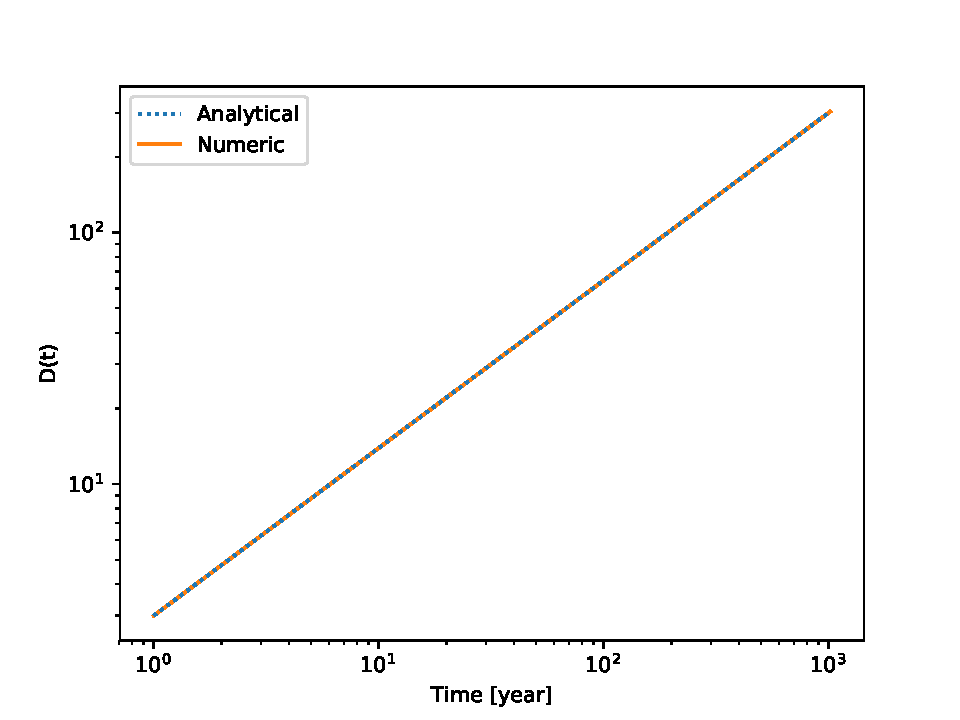
\includegraphics[width=14cm, height=8.5cm]{./Plots/3_ode_0.pdf}
\caption{The analytical (blue) and numerical (orange) solution of the ODE with initial conditions $D(1) = 3, D'(1) = -10$. The plots show that he numerical solution does not appear to have a visible deviation from the analytical solution for the given time interval.}
\end{figure}

\begin{figure}[!ht]
\centering
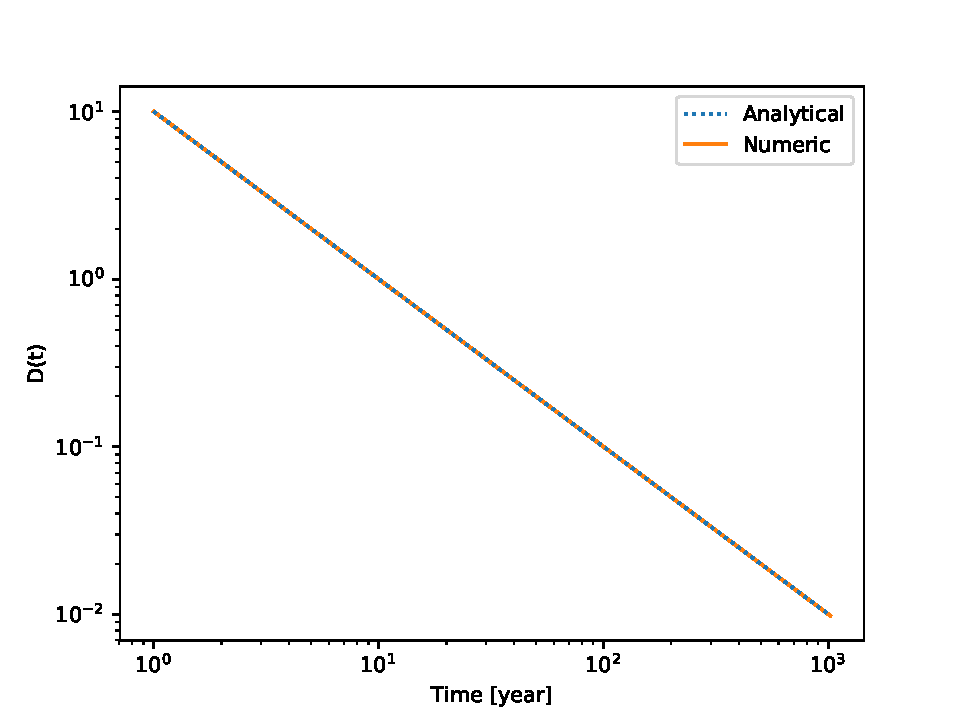
\includegraphics[width=14cm, height=8.5cm]{./Plots/3_ode_1.pdf}
\caption{The analytical (blue) and numerical solution (orange) of the ODE with initial conditions $D(1) = 10,  D'(1) = -10$. The plots show that he numerical solution does not appear to have a visible deviation from the analytical solution for the given time interval.}
\end{figure}
\newpage


\begin{figure}[!ht]
\centering
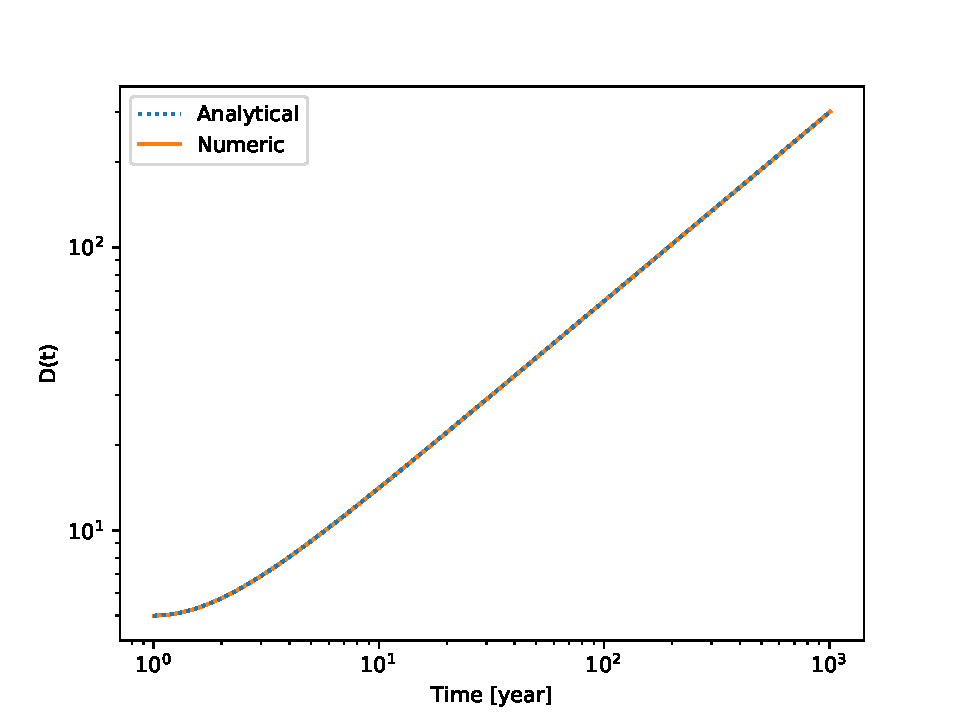
\includegraphics[width=14cm, height=8.5cm]{./Plots/3_ode_2.pdf}
\caption{The analytical (blue) and numerical (orange) solution of the ODE with initial conditions $D(1) = 5,  D'(1) = 0$. The plots show that he numerical solution does not appear to have a visible deviation from the analytical solution for the given time interval.}
\end{figure}

\end{quote}
\end{quote}






